% !TeX root = main.tex
\section{Results}
\label{sec:results}

\subsection{Simulation variables}
The following simulation variables were set. Except mass, all others were assumed.

\lstinputlisting[language=python, firstline=21, lastline=62]{./../python/uav_move.py}

The total code is present in Appendix \ref{app:code-uav-motion}. The remainder of this section presents graphs generated by the code. Note that each target has the initial conditions as above (zero).

It is also interesting to observe that all items settle to zero in the end, except the thrust to counter weight (which is reflected in the desired acceleration, thrust, and even the actual motor speeds).

\pagebreak
\subsection{Target 1: (20, 40, -5)}

\begin{figure}[h]
    \centering
    % Position and velocity
    \begin{subfigure}[b]{0.35\textwidth}
        \includegraphics[width=\textwidth]{pos1/position.jpg}
    \end{subfigure}
    \begin{subfigure}[b]{0.35\textwidth}
        \includegraphics[width=\textwidth]{pos1/velocity.jpg}
    \end{subfigure}
    % Acceleration (actual and desired)
    \begin{subfigure}[b]{0.35\textwidth}
        \includegraphics[width=\textwidth]{pos1/acceleration.jpg}
    \end{subfigure}
    \begin{subfigure}[b]{0.35\textwidth}
        \includegraphics[width=\textwidth]{pos1/acceleration_d.jpg}
    \end{subfigure}
    % Euler angles
    \begin{subfigure}[b]{0.35\textwidth}
        \includegraphics[width=\textwidth]{pos1/euler.jpg}
    \end{subfigure}
    \begin{subfigure}[b]{0.35\textwidth}
        \includegraphics[width=\textwidth]{pos1/euler_d.jpg}
    \end{subfigure}
    % Desired thrust and motor speeds
    \begin{subfigure}[b]{0.35\textwidth}
        \includegraphics[width=\textwidth]{pos1/thrust_d.jpg}
    \end{subfigure}
    \begin{subfigure}[b]{0.35\textwidth}
        \includegraphics[width=\textwidth]{pos1/motor_speeds.jpg}
    \end{subfigure}
    \caption{Plots for $\mathbf{x}_d = [20\;\;40\;\;-5]^\top$}
    \small
        The \emph{first} row has actual position and velocity.
        The \emph{second} row has actual and desired acceleration.
        The \emph{third} row has actual and desired euler angles (euler, w.r.t. ground/world frame).
        The \emph{fourth} row has the thrust desired (to counter weight) and the motor speeds.
\end{figure}

\pagebreak
\subsection{Target 2: (30, -50, -5)}

\begin{figure}[h]
    \centering
    % Position and velocity
    \begin{subfigure}[b]{0.35\textwidth}
        \includegraphics[width=\textwidth]{pos2/position.jpg}
    \end{subfigure}
    \begin{subfigure}[b]{0.35\textwidth}
        \includegraphics[width=\textwidth]{pos2/velocity.jpg}
    \end{subfigure}
    % Acceleration (actual and desired)
    \begin{subfigure}[b]{0.35\textwidth}
        \includegraphics[width=\textwidth]{pos2/acceleration.jpg}
    \end{subfigure}
    \begin{subfigure}[b]{0.35\textwidth}
        \includegraphics[width=\textwidth]{pos2/acceleration_d.jpg}
    \end{subfigure}
    % Euler angles
    \begin{subfigure}[b]{0.35\textwidth}
        \includegraphics[width=\textwidth]{pos2/euler.jpg}
    \end{subfigure}
    \begin{subfigure}[b]{0.35\textwidth}
        \includegraphics[width=\textwidth]{pos2/euler_d.jpg}
    \end{subfigure}
    % Desired thrust and motor speeds
    \begin{subfigure}[b]{0.35\textwidth}
        \includegraphics[width=\textwidth]{pos2/thrust_d.jpg}
    \end{subfigure}
    \begin{subfigure}[b]{0.35\textwidth}
        \includegraphics[width=\textwidth]{pos2/motor_speeds.jpg}
    \end{subfigure}
    \caption{Plots for $\mathbf{x}_d = [20\;\;40\;\;-5]^\top$}
    \small
        The \emph{first} row has actual position and velocity.
        The \emph{second} row has actual and desired acceleration.
        The \emph{third} row has actual and desired euler angles (euler, w.r.t. ground/world frame).
        The \emph{fourth} row has the thrust desired (to counter weight) and the motor speeds.
\end{figure}

\pagebreak
\subsection{Target 3: (-10, -60, -5)}

\begin{figure}[h]
    \centering
    % Position and velocity
    \begin{subfigure}[b]{0.35\textwidth}
        \includegraphics[width=\textwidth]{pos3/position.jpg}
    \end{subfigure}
    \begin{subfigure}[b]{0.35\textwidth}
        \includegraphics[width=\textwidth]{pos3/velocity.jpg}
    \end{subfigure}
    % Acceleration (actual and desired)
    \begin{subfigure}[b]{0.35\textwidth}
        \includegraphics[width=\textwidth]{pos3/acceleration.jpg}
    \end{subfigure}
    \begin{subfigure}[b]{0.35\textwidth}
        \includegraphics[width=\textwidth]{pos3/acceleration_d.jpg}
    \end{subfigure}
    % Euler angles
    \begin{subfigure}[b]{0.35\textwidth}
        \includegraphics[width=\textwidth]{pos3/euler.jpg}
    \end{subfigure}
    \begin{subfigure}[b]{0.35\textwidth}
        \includegraphics[width=\textwidth]{pos3/euler_d.jpg}
    \end{subfigure}
    % Desired thrust and motor speeds
    \begin{subfigure}[b]{0.35\textwidth}
        \includegraphics[width=\textwidth]{pos3/thrust_d.jpg}
    \end{subfigure}
    \begin{subfigure}[b]{0.35\textwidth}
        \includegraphics[width=\textwidth]{pos3/motor_speeds.jpg}
    \end{subfigure}
    \caption{Plots for $\mathbf{x}_d = [20\;\;40\;\;-5]^\top$}
    \small
        The \emph{first} row has actual position and velocity.
        The \emph{second} row has actual and desired acceleration.
        The \emph{third} row has actual and desired euler angles (euler, w.r.t. ground/world frame).
        The \emph{fourth} row has the thrust desired (to counter weight) and the motor speeds.
\end{figure}

\pagebreak
\subsection{Target 4: (-70, 30, -5)}

\begin{figure}[h]
    \centering
    % Position and velocity
    \begin{subfigure}[b]{0.35\textwidth}
        \includegraphics[width=\textwidth]{pos4/position.jpg}
    \end{subfigure}
    \begin{subfigure}[b]{0.35\textwidth}
        \includegraphics[width=\textwidth]{pos4/velocity.jpg}
    \end{subfigure}
    % Acceleration (actual and desired)
    \begin{subfigure}[b]{0.35\textwidth}
        \includegraphics[width=\textwidth]{pos4/acceleration.jpg}
    \end{subfigure}
    \begin{subfigure}[b]{0.35\textwidth}
        \includegraphics[width=\textwidth]{pos4/acceleration_d.jpg}
    \end{subfigure}
    % Euler angles
    \begin{subfigure}[b]{0.35\textwidth}
        \includegraphics[width=\textwidth]{pos4/euler.jpg}
    \end{subfigure}
    \begin{subfigure}[b]{0.35\textwidth}
        \includegraphics[width=\textwidth]{pos4/euler_d.jpg}
    \end{subfigure}
    % Desired thrust and motor speeds
    \begin{subfigure}[b]{0.35\textwidth}
        \includegraphics[width=\textwidth]{pos4/thrust_d.jpg}
    \end{subfigure}
    \begin{subfigure}[b]{0.35\textwidth}
        \includegraphics[width=\textwidth]{pos4/motor_speeds.jpg}
    \end{subfigure}
    \caption{Plots for $\mathbf{x}_d = [20\;\;40\;\;-5]^\top$}
    \small
        The \emph{first} row has actual position and velocity.
        The \emph{second} row has actual and desired acceleration.
        The \emph{third} row has actual and desired euler angles (euler, w.r.t. ground/world frame).
        The \emph{fourth} row has the thrust desired (to counter weight) and the motor speeds.
\end{figure}
